\section{1.2}

\textit{Hvilket slags spil vil vi lave?}\\

Vi sigtede i gruppen efter at lave et simpelt spil, hvor fokus kunne ligge på programmeringen i scratch i stedet for at bruge en masse tid på gamedesign.\\

Simpel hop over forhindringer i 2d sidecrolling miljø!

\subsection{Spilkoncept}

Katten skal undgå at blive bidt af hunden ved at hoppe over hunden. Hver gang man hopper over hunden får man et point, der tælles oppe i venstre hjørne. Hundens hastighed øges ydermere for hver point man scorer. Dette skaber en dynamisk sværhedsgrad der tilpasser spillerens evne.\\

\begin{figure}[ht]
	\centering
	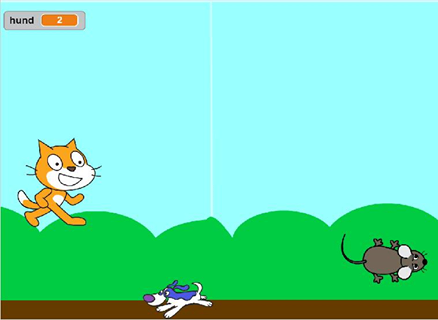
\includegraphics[scale=0.5]{Scratch_Game.png}
	\caption{{Scratch Spil}}
	\label{fig:screen_dump}
\end{figure}

\clearpage
\subsection{Programmering}

Som den mest fundamentale funktion i spillet skal katten kunne hoppe over hunden.\\

\begin{figure}[ht]
	\centering
	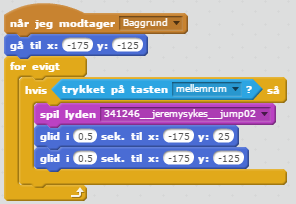
\includegraphics[scale=1]{jump.png}
	\caption{{Hoppe mekanismen for katten}}
	\label{fig:jumpCat}
\end{figure}

Når katten modtager startmeddelelsen (Baggrund), vil den altid antage sin startposition givet ved koordinaterne (x:-175, y:-125). Derefter vil den for evigt vente på spilleren giver kommandoen mellemrum, hvor efter den i et bestemt tidsinterval vil rykke hundred enheder op på y og ned.\\

Dernæst skal vores kat holde øje med om den støder ind i hunden.\\

\begin{figure}[ht]
	\centering
	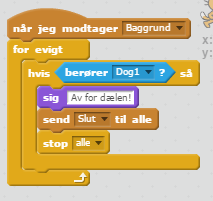
\includegraphics[scale=1]{collision.png}
	\caption{{Kollision med hunden}}
	\label{fig:coll}
\end{figure}

Når spriten modtager vores startmeddelelse holder katten for evigt øje med om den berør en hund. Hvis katten på et vilkårligt tidspunkt berør hunden siger den 'Av for dælen!' og vil dernæst sende en besked rundt som får Game over-spriten til at dukke op, inden den stopper alle andre scripts.\\
\clearpage
Vores spil er også afhængigt af at der skabes hunde som katten undgå\\

\begin{figure}[ht]
	\centering
	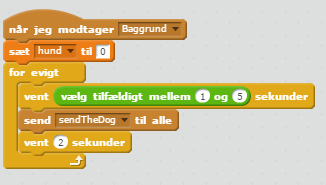
\includegraphics[scale=1]{baggrunddog.png}
	\caption{{Sender signal ved tilfældige intervaller til at skabe og sende hunde}}
	\label{fig:dog_sig}
\end{figure}

Når startmeddelelsen sendes rundt, nulstilles vores hundevariabel for det første, idet den angiver hvor mange hunde man har undgået. Derefter vil hundene resten af spillet skabes i et interval på 1-5 + 2 sekunder, de to sekunder er lagt til for at sikre en hvis reaktionstid for spilleren. Når en hund skal skabes sendes beskeden 'sendTheDog'. (Vi kunne dog have ændret det tilfældige valg til 3-7 sekunder og opnå samme resultat som ved at fjerne en vent 2 sekunder block)\\

\begin{figure}[ht]
	\centering
	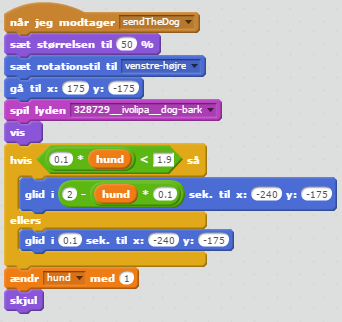
\includegraphics[scale=1]{sendthedog.png}
	\caption{{Initialisere hunden og bestemmer hastigheden på baggrund af point}}
	\label{fig:dog_init}
\end{figure}

Metoden for glideanimationen af hunden fra højre til venstre starter når signalet 'sendTheDog' bliver modtaget. Først bliver hundens størrelse, retning og startposition angivet for så at afspille en "wow" lyd og vise hunden. Dernæst skal hunden glide 0.1 sekunder hurtigere for hver hund man hopper over. Der er sat en begrænsning hvor hunden minimalt vil glide gennem banen med 0.1 sekunder. 
